%%% Made of Tiny Robots
%%% An Investigation of the Ecology of Responsive Environments
%%%
\chapter{An Ontology of Responsive Environments}
\label{ch:ontology}
%
As we enter the age of ubiquitous computing \citep{weiser_1999} our relationship with our artifact ecology is changing. 
There are several factors to these changes: we have new ways to fabricate artifacts; we have new ways of relating to artifacts; and our artifacts increasingly perform tasks that were once the exclusive domain of people.
One of the key changes in an artifact ecology (that drives other changes) is the emergence of powerful computational agents that manage the explosion of relationships (and data) that arise when every artifact begins to communicate over the network.
Many of these computational artifacts feed into online data stores physically situated in massive computing clusters (which we will refer to generally as \emph{temples}\footnote{Because they are capable of hosting idols such as the googlebot.}), managed by agents like the googlebot (which we will refer to generally as \emph{idols}\footnote{We chose the name `idol' after Gibson's `idoru'\citeyearpar{gibson_idoru}, a literal AI rock star, with the accompanying cultural leverage of a teen idol; and after religious idols, to draw an analogy with the religious practice of asking powerful ethereal agents for advice and favors.}).

As we enter into a cybernetic relationship with this new artifact ecology much of what we have until now considered our private personas will be determined by the behavior of the robotic devices we surround ourselves with, and by our relationship with the idols that manage these devices and mediate our interactions with other people, as we discuss in section~\ref{sec:idols}.
The character of this ecology, and what it means to be and individual within this new order, will depend largely on two factors: the transparency of these mechanisms to individuals, and their reconfigurability.

As our focus is not idols themselves but how our artifact ecology can be arranged to interface with them, in section~\ref{sec:kinds_of_artifacts} we will discuss what kinds of artifacts can be found in a responsive environment.
In section~\ref{sec:artifact_ecologies} we will describe several possible responsive environment ecologies in which such artifacts could be produced and deployed. 
In an attempt to support the development of systems that support transparency and reconfigurability, we will focus on what we are calling a robunculi ecology: where rather than acquiring finished products people largely acquire robotic kits of parts that can either be assembled, or can self-assemble, into a variety of forms on demand. 
We will discuss the opportunities that this artifact ecology provides for a wide spectrum of society to play a role in shaping the behavior of their environment. 

In section~\ref{sec:robunculi_ontology} we will look in more detail at the roles people can play within a robunculi ecology, and at the methods people adopting various roles can use to interact with these systems, by developing an ontology of interaction modes. We suggest that many of these interaction modes could also be usefully applied within other artifact ecologies to provide transparency and reconfigurability.

Finally in section~\ref{sec:ecological_impacts} we describe some potential impacts of the adoption of different responsive environment ecologies, and highlight tensions that we will refer back to in our survey of robunculi in chapter~\ref{ch:survey}, and in our more detailed case studies in chapter~\ref{ch:case_studies}.

\section{Idols}
\label{sec:idols}
%
While we have related to our leveraged environments primarily as tool-users, as our environment becomes responsive this relationship is becoming more of a partnership amongst ourselves and various computational agents. 
For example in a leveraged environment professionals would often supplement their memory by using a notebook and appointment book, and supplement their expertise with a small private library. 
In a responsive environment, professionals supplement their memory through a small computer carried on their person (which we will call a \emph{crystal}\footnote{We call this class of handheld computers that provide a constant connection to the network `crystals', as in a crystal ball that is used to view distant places and communicate with other agents through the ether, and as a reference to their current popular physical realization as a fragile glass-plated touchscreen.}) that manages notes and appointments through the interaction of a variety of software agents over a network; they supplement their expertise by using this same device to query an idol (i.e. the googlebot).
Of course professionals in a leveraged environment also practice division of labor, with secretaries managing appointments and engineers on call to make judgements using their personal libraries to supplement their domain knowledge.
The difference is that in a leveraged environment partnerships are between people, and artifacts only effect change when operated by a person.
Now when people send us invitations (from their crystals, over the network) an idol helpfully inserts them into our calendars and then buzzes us through our own crystals at the appropriate time to tell us where to be.

We suggest that the outlook for accepting these idols into our cybernetic consciousness varies from the utopian to the orwellian largeley depending on: how much control we (the citizens of idol-mediated societies) have over the behavior of our devices and idols; and how transparent (to us) the mechanisms governing these behaviors are. But before we can discuss the qualities of these computational artifacts we should discuss what kinds of artifacts we expect to see.

\section{Kinds of Artifacts}
\label{sec:kinds_of_artifacts}
%
\begin{figure}[h!]
  \centering
%    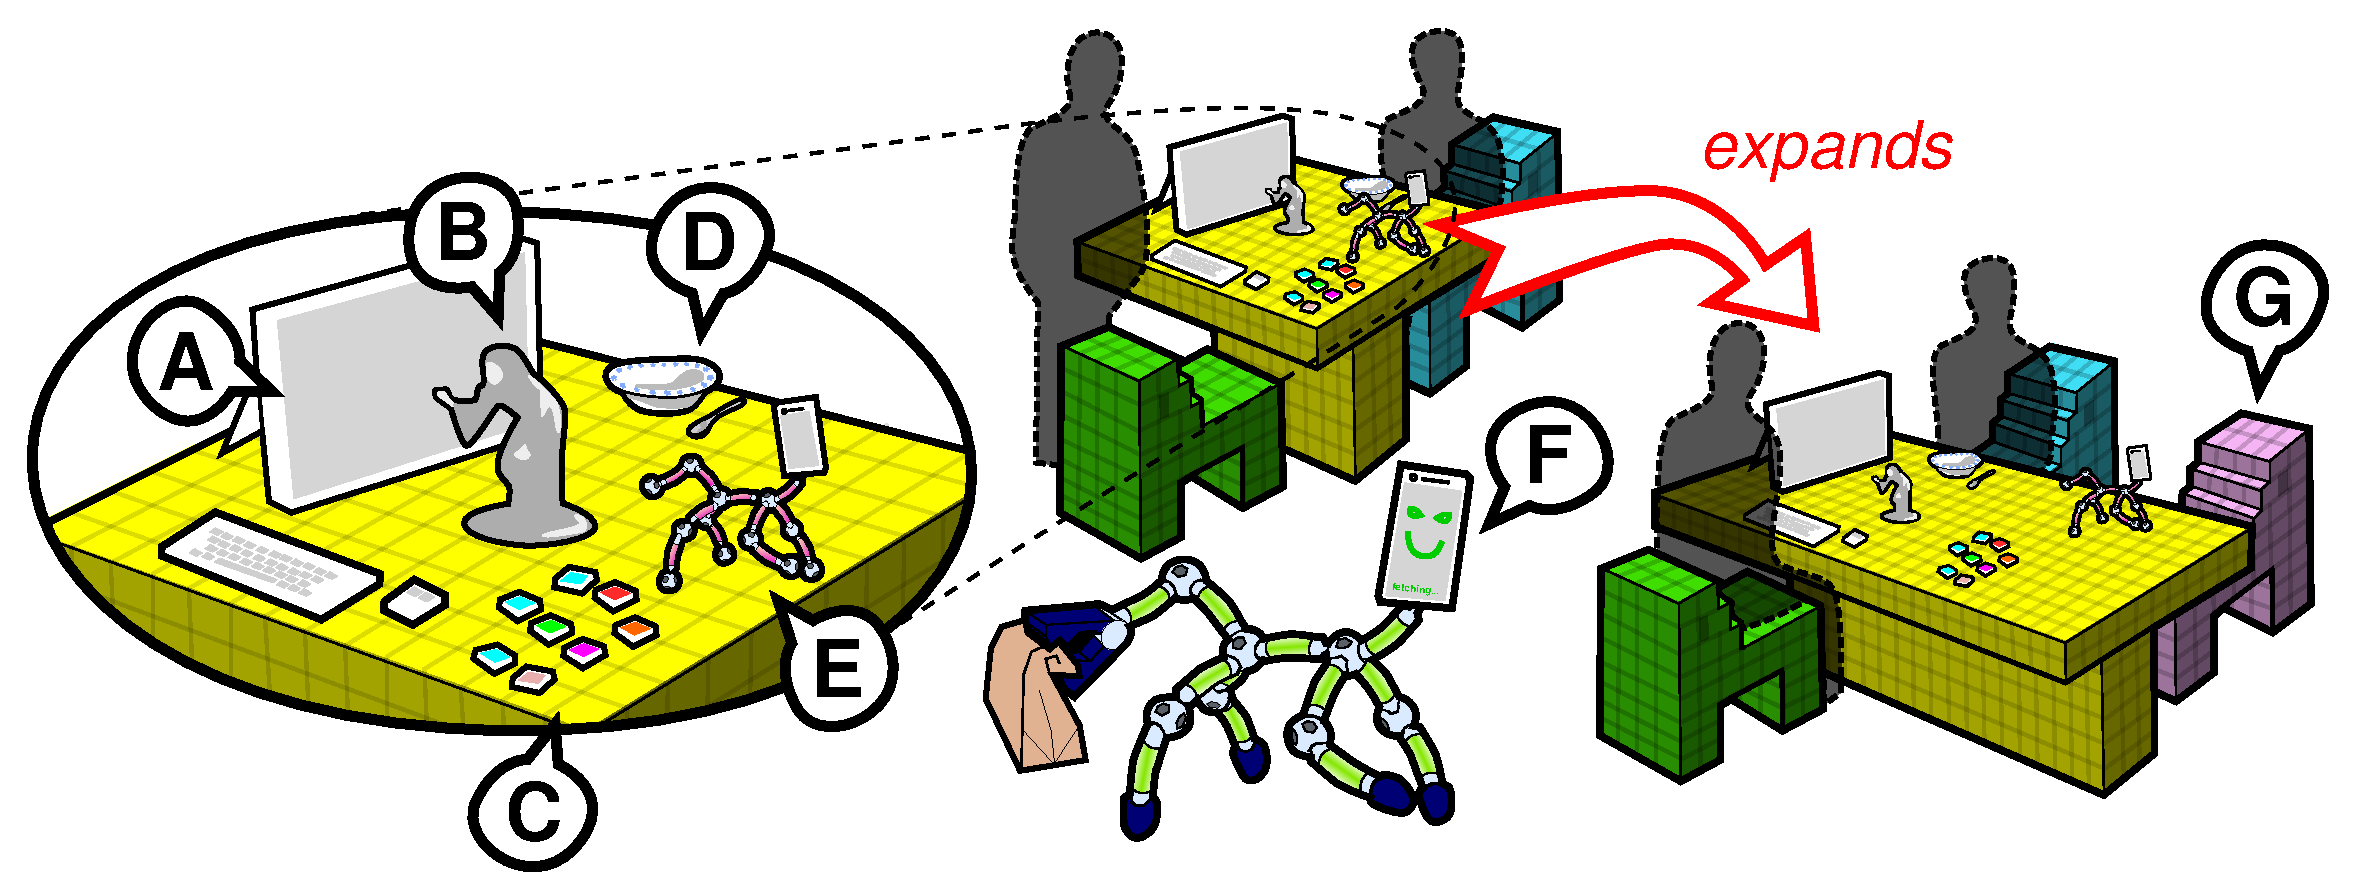
\includegraphics[width=\textwidth]{kinds_of_artifacts.pdf}
    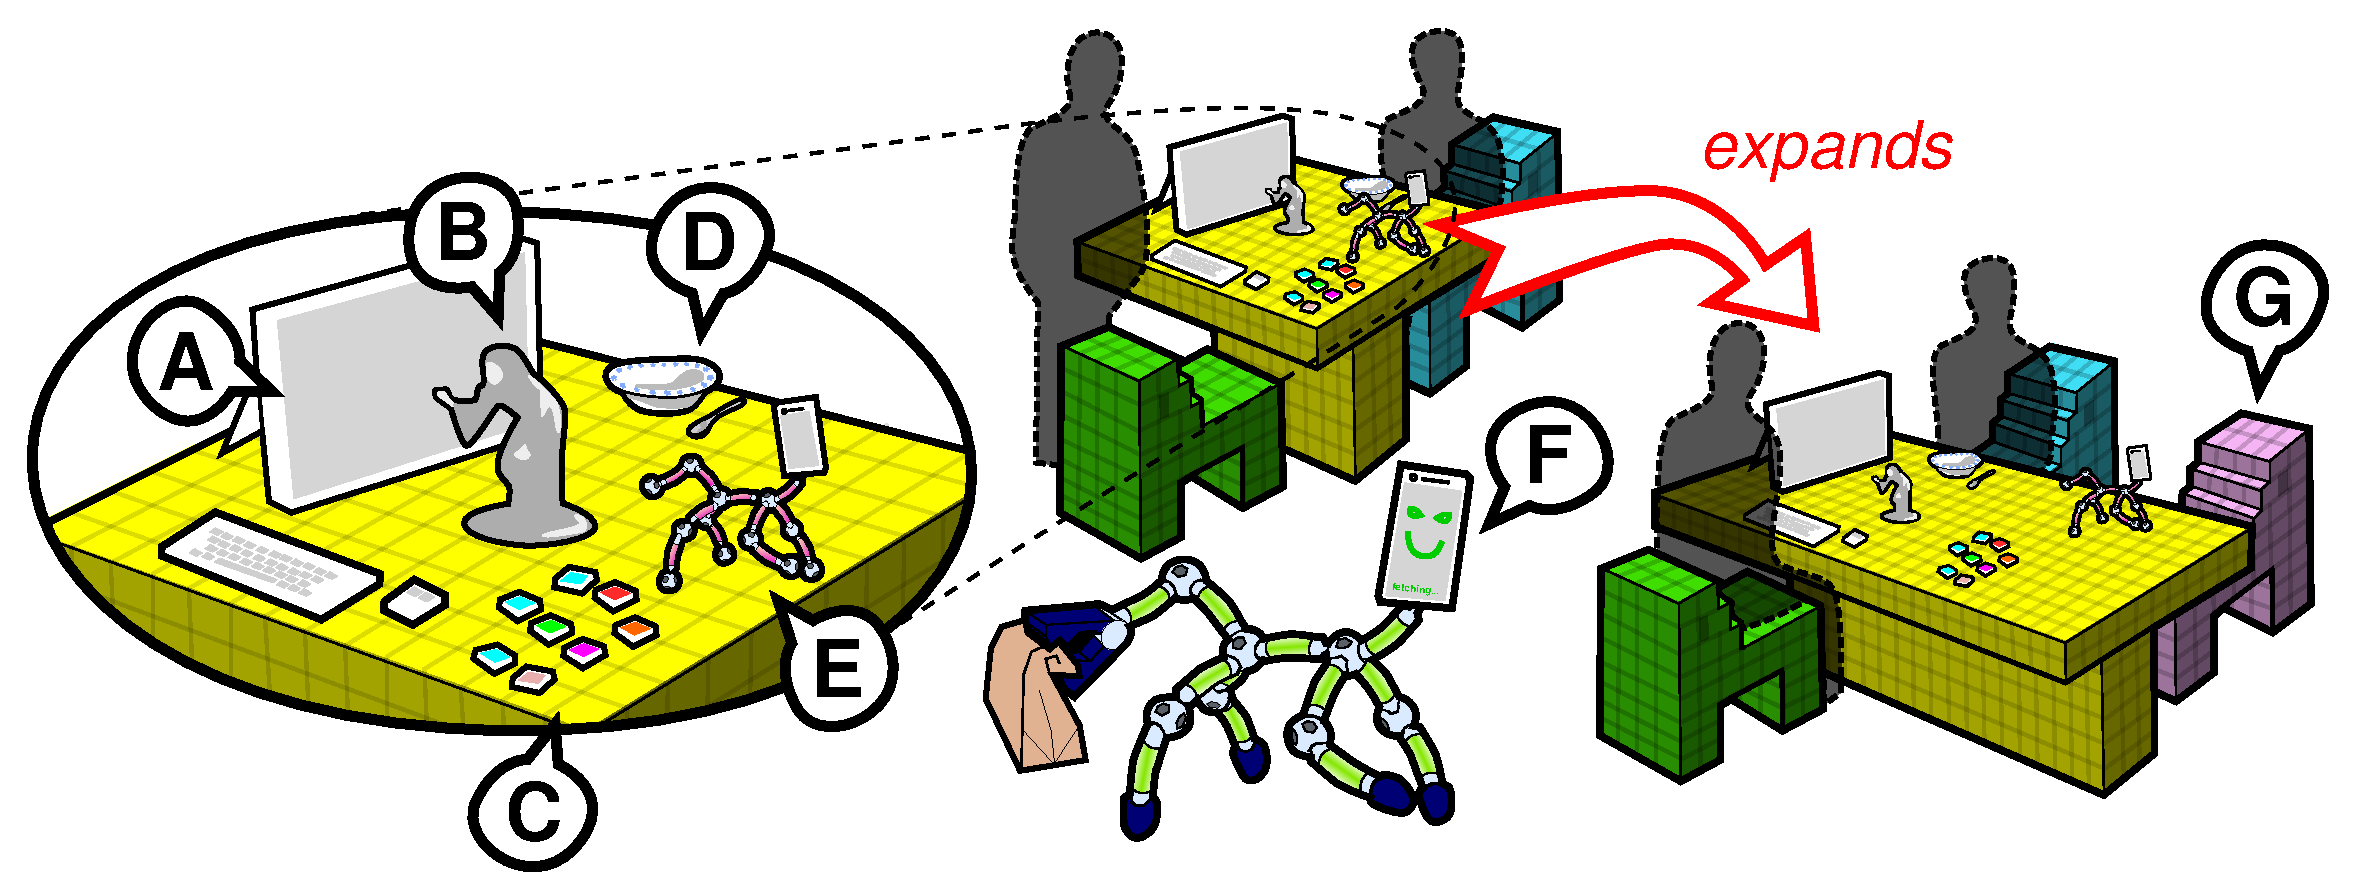
\includegraphics[width=125mm]{kinds_of_artifacts.pdf}
  \caption{An illustration of various kinds of artifacts found in responsive environments: \emph{A)} a (work)bench computer (a popsicle); \emph{B)} an avatar hyperthou; \emph{C)} a tile tinkit; \emph{D)} a bowl and spoon (duckcicles); \emph{E)} a stickpuppet fig (with a hub-and-strut tinkit body and a volticle crystal for a head); \emph{F)} a golem fig fetching lunch; \emph{G)} a social table hyperfig (composed of prismatic cube bunkles) that expands as people sit to keep an empty chair available by drawing more bunkles from a reservoir.}
  \label{fig:kinds_of_artifacts}
\end{figure}
%


\begin{figure}[tb]
  \centering
    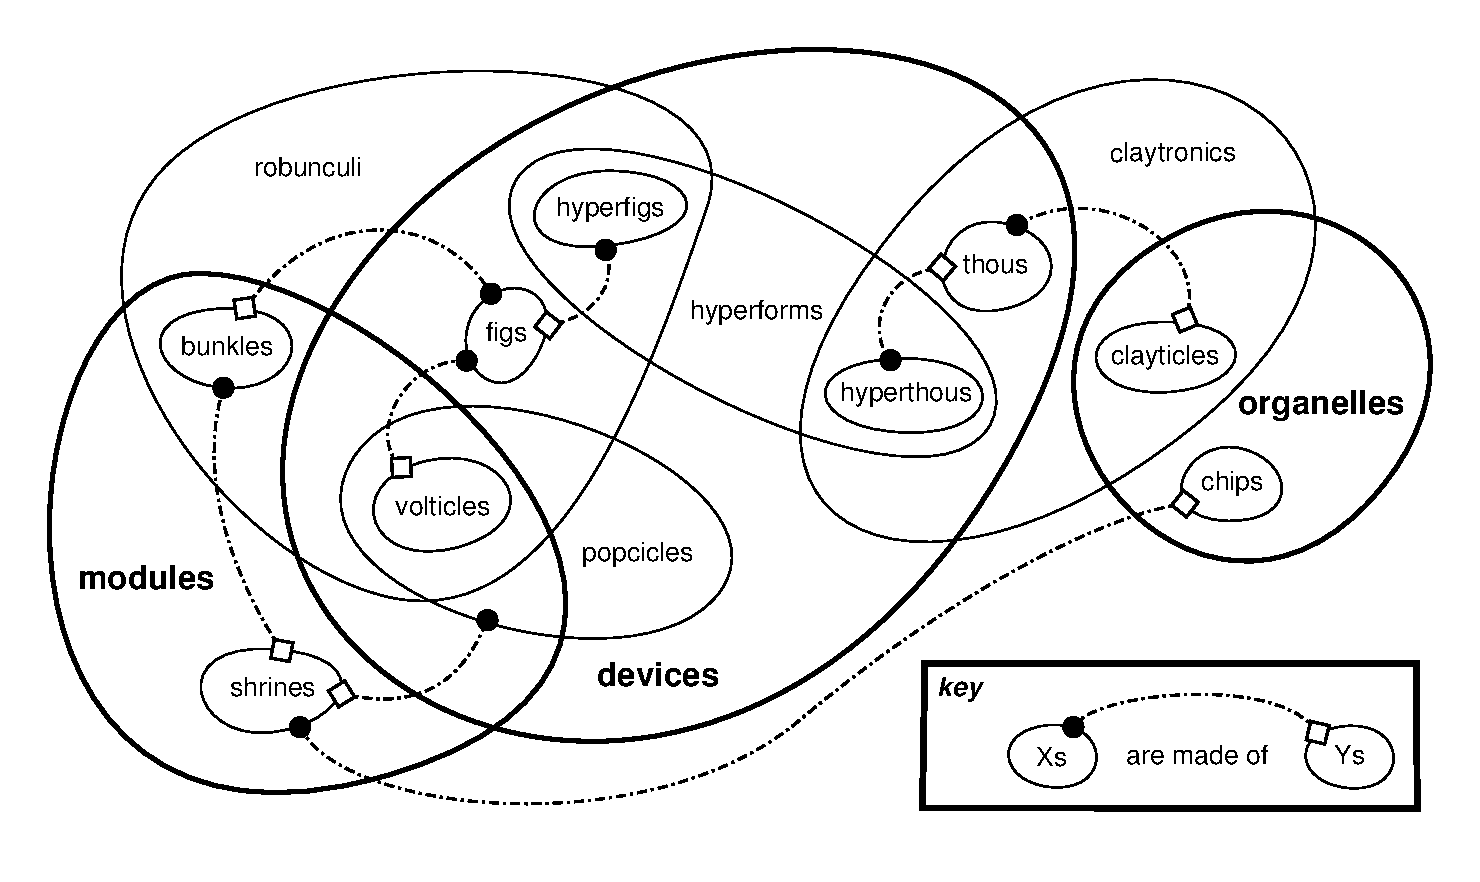
\includegraphics[width=140mm]{hardware_venn.pdf}
  \caption{Venn diagram of the different categories of computational artifacts.}
  \label{fig:hardware_venn}
\end{figure}

    \begin{enumerate}
        \item construction kits vs rapid prototyping
        \item robunculi, productization and reuse
    \end{enumerate}


[TODO: figures showing axes] (transparency - physically secured state/corp rental -> drm'd black box -> open source hardware) (reconfigurability - mass-manufactured widget -> bespoke popsicle -> kit of parts -> hyperform)


\section{Examples of Artifact Ecologies}
\label{sec:artifact_ecologies}
%
\subsection{nodes of power}
        \begin{enumerate}
            \item manufacturing
            \item data transmission
            \item data stores
            \item shrines (high-powered computing clusters)
            \item leaf node control
        \end{enumerate}        


\section{Robunculi: an Ontology}
\label{sec:robunculi_ontology}
    \begin{enumerate}
        \item robunculi typologies
        \begin{enumerate}
            \item idols
            \item tangible sketches
            \item golems
            \begin{enumerate}
                \item sock puppet (dumb rc golem)
                \item avatar (golem serving as interface to idol)
            \end{enumerate}
            \item hyperforms
        \end{enumerate}
        \item morphologies
        \begin{enumerate}
            \item tile
            \item block
            \item skeleton (graph)
            \item panel
            \item glass (screen / projection interface)
            \item shrine (idol-scale computing facility)
        \end{enumerate}
        \item affordances
        \begin{enumerate}
            \item parallel affordances are synergistic
            \item placing / self-reconfiguring
            \item posing / flexing (self-posing)
            \item commanding (pointing) / signalling (haloing)
            \item listening (tagging) / responding (texting)
            \item graffing (accepting drawings) / gramming (responding with drawings)
            \item puppeteering / puppeting (present puppeteering interface)
            \item sinks generate structured data to be accessed through idols
            \item logging (recording interactions to data stores) (sink)
            \item crawling (indexing data stores) (sink)
            \item tracking (id-ing and classifying agents with sensors) (sink)
            \item slamming (exploring and mapping environments) (sink)
        \end{enumerate}
    \end{enumerate}


\section{Potential (Artifact) Ecological Impacts of Responsive Environments}
\label{sec:ecological_impacts}
%
    \begin{enumerate}
        \item radical transparency - big brother and little brother
        \item means of production 2 - factories vs 3d printers
        \item battle of the heavens - corporate clouds vs govt clouds vs community clouds
        \item digital serfdom and device transparency
    \end{enumerate}



